\documentclass[a4paper,12pt, openany]{report}
\usepackage[utf8]{inputenc}
\usepackage[T1]{fontenc}
\usepackage[a4paper,left=2cm,right=2cm,top=2cm,bottom=2cm]{geometry}
\usepackage[frenchb]{babel}
\usepackage{enumitem}
\usepackage[pdftex]{graphicx}
\usepackage{xcolor}
\usepackage{soul}
\usepackage{import} 
\usepackage{hyperref}
\setlength{\parindent}{0cm}
\setlength{\parskip}{1ex plus 0.5ex minus 0.2ex}
\newcommand{\hsp}{\hspace{20pt}}
\newcommand{\HRule}{\rule{\linewidth}{0.5mm}}
\newtheorem{definition}{Définition}[section]
\colorlet{mdtRed}{red!50!black}
\renewcommand\thesection{\arabic{section}}
\setcounter{secnumdepth}{3}
\setcounter{tocdepth}{3}
\setlength{\parindent}{0.7cm}
\usepackage{enumitem}
\usepackage{amsmath}
\usepackage{amsfonts}
\usepackage{amssymb}
\usepackage{amsthm}
\usepackage{caption}
\usepackage{lettrine}
\usepackage{hyperref}
\usepackage{graphicx}
\usepackage{booktabs}
\usepackage{float}
\usepackage{smartdiagram}
\usepackage{fancyhdr}
\usepackage{afterpage}
\usepackage{mathtools}
\usepackage{mathrsfs}
\usepackage{mathptmx}
\usepackage{bm}
\usepackage{pdfpages}
\usepackage{algorithmic}
\usepackage{algorithm}
\renewcommand{\mathbf}[1]{\textbf{\mathversion{bold}$#1$}}
\renewcommand{\textbf}[1]{\begingroup\bfseries\mathversion{bold}#1\endgroup}
\pagestyle{fancy}
\lhead{}
\chead{}
\rhead{\leftmark}
\lfoot{\small Projet IFT712 }
\cfoot{\thepage}
\rfoot{\small 2019-2020}
\renewcommand{\headrulewidth}{0.4pt}
\renewcommand{\footrulewidth}{0.4pt}

\begin{document}

\begin{titlepage}
    \begin{center}
        
\includegraphics[width=3cm, height=3cm, keepaspectratio]{udes.png}
        \centering
        \vspace*{.06 \textheight}
        
        
        % Nom de l'école 
        {
            \scshape \LARGE{\color{mdtRed}Univérsité de Sherbrooke} \par
        }
        \vspace{1.5cm}
        
        % Type du projet
        \textsc {
            \Large Projet IFT 712 \\
            \vspace{0.2cm}
            Informatique - Deuxième cycle
        } \\ [1cm]
        
        % Titre du projet
        \HRule \\ [0.4cm]
        {
            \huge \bfseries \textsc{{Méthodes de classification par Sklearn\\}}
        }
        \vspace{0.4cm}
        \HRule \\ [1.5cm]
         
        
        \begin{minipage}[t]{0.4\textwidth}
            \begin{flushleft} 
                \large \emph {Réalisé par:} \\
                \vspace{0.05cm}
                { \color{mdtRed}
                    {\textsc{THOUIN} Kevin } \\    
                    {\textsc{BENNANI} Kaoutar} \\
                }
            \end{flushleft}
        \end{minipage}
        \begin{minipage}[t]{0.4\textwidth}
            \begin{flushright} \large
                \emph{Supervisé par:} \\
                {\color{mdtRed} Pr. Pierre-Marc JODOIN}\\
            \end{flushright}
        \end{minipage}\\[4cm]
        
        {\large Année universitaire 2019 - 2020}\\[4cm]
         
        \vfill
    \end{center}
\end{titlepage}
\clearpage


\tableofcontents
\clearpage

\addcontentsline{toc}{chapter}{Table des figures}
\listoffigures
\clearpage


 \chapter{Présentation du projet}
\section{Présentation}
\par Ce projet de session fait partie des travaux du cours IFT712, il a pour objectif de tester quelques méthodes de classification sur une base de données
Kaggle (www.kaggle.com) avec la bibliothèque Sklearn .
\section{Choix de la base de données}
\par Nous avons choisi comme base de données: "Wine Dataset".
\par A propos de la base de données, les données sont le résultat d'une analyse chimique de vins cultivés dans une des régions d'Italie mais issus de trois cultivars différents.
\par Parmi ses caracteristiques:
\begin{itemize}[label=\textbullet]
    \item 178 instances
    \item 13 variables
    \item les valeurs des attributs sont des Integer et des Float
    \item Pas de valeurs manquantes
    \item Généralement utilisé pour les tâches de classification
\end{itemize}
\section{Choix du design}
\par Le projet contient 8 classes en total.
\begin{itemize}[label=\textbullet]
    \item La classe 'Classification\_main.py'
    \item La classe 'Classification\_neural\_net.py': Décrit l'algorithme de classification par réseau de neurones.
    \item La classe 'Classification\_logistique.py': S'agit de la classification par régréssion logistique.
    \item La classe 'Classification\_bagging.py': Classification par l'algorithme Bagging.
    \item La classe 'Classification\_adaboost.py': Classification par l'algorithme AdaBoost.
    \item La classe 'Classification\_svm.py': Il s'agit du code correspondant au SVM.
    \item La classe 'Classification\_hyperparameter.py': Il s'agit des techniques de la recherche des hypers paramètres pour chacun des algorithmes de classification.
    \item La classe 'Classification\_io.py': Cette classe crée des données d"entrainement et de test à partir du "Wine Dataset" et a une fonction permettant l'affichage graphique.
\end{itemize}
\section{Gestion du projet}
\par Pour la réalisation du projet, nous avons utilisé le gestionnaire de version de code "git" via la plateforme "gitHub"

 \chapter{Les algorithmes et démarche utilisés}
\par Cette partie consiste à présenter les algorithmes utilisés, ainsi que la démarche scientifique suivie.
\section{Algorithmes}
Les algorithmes utilisés sont:
\begin{itemize}[label=\textbullet]
\item Régression logistique : les hyperparamètres sont le terme de régularisation et le taux d'apprentissage. Cette algorithme devrait bien performé si les données
    sont linéairement séparable, ce qui est une hypothèse peut-être audacieuse.
\item SVM : Nous utilisons le noyau rbf. Nous n'avons pas d'hyperparamètres pour cette algorithme de classification.
\item Réseaux de neuronnes: Nous testons avec une ou deux couches de six neuronnes. Les hyperparamètres sont la fonction d'activation (relu ou logistique), le terme
    de régularisation, le taux d'apprentissge et le momentum pour la descente de gradient.
\item Bagging : Nous avons deux hyperparamètres. Le premier est l'estimateur (adaboost ou un réseau de neurones avec des couches de six neurones), le second est le
    nombres d'estimateurs
\item AdaBoost : Nous utilisons un arbre de décision de profondeur un comme estimateur de base. Nous avons deux hyperparamètres. Le premier est le nombre
    d'estimateurs et le second est le taux d'apprentissage
\end{itemize}

\section{Démarche scientifique}
\subsection{Organisation des données}
\par Aprés la récupération des données du "Wine Dataset", on a divisé ces données en des données d'entrainement et des données de test. Cela se voit dans la classe: "Classification\_io.py". Avant de les utiliser, nous avons centré et réduit celles-ci. Nous avons fait attention à n'utiliser que les données d'entrainement pour trouver
la transformation.
\par Donc, l'entrainement et le test ont été fait sur deux données différentes: x\_train et x\_test.
\subsection{Cross-validation}

\subsection{Recherche des hyper-paramètres}
\par La classe "Classification\_hyperparameter.py" est notre implémentation de la méthode de la recherche des hyper-paramètres. Ceci a été fait à l'aide de "GridSearchCV" de la biblithèque "sklearn.model\_selection"




 \chapter{Analyse des résultats}
\par Dans cette partie nous allons analyser les résultats de chacun des algorithmes.
\section{Résultats}
\subsection{Régression logistique}
\begin{figure}[H]
    \centering
    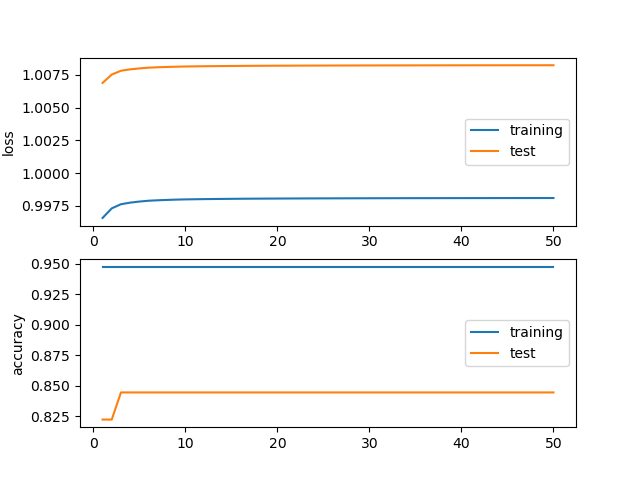
\includegraphics[width=17cm, height=10cm, keepaspectratio]{logistique_plot.png}
    \caption{Figure diagrames "accuracy" et "loss" pour la régression logistique }
    \label{Figure diagrames "accuracy" et "loss" pour la régression logistique  }
\end{figure}
\par Pour "lr" entre 0.0001 et 0.001, et pour "l2reg" entre 0.1 et 10, les meilleurs valeurs pour les hyper-paramètres "lr" et "l2reg" sont ceux affichés dans la figure ci-dessous
\begin{figure}[H]
    \centering
    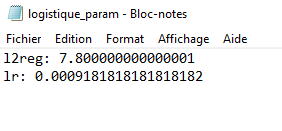
\includegraphics{logistique_param.PNG}
    \caption{Figure parametres de régression logistique}
    \label{Figure parametres de régression logistique }
\end{figure}
\subsection{SVM}
\par Les erreurs et les précisions d'entrainement et de test:
\begin{figure}[H]
    \centering
    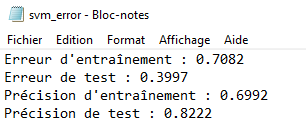
\includegraphics{svm.png}
    \caption{Figure SVM-error }
    \label{Figure fichier svm-error }
\end{figure}
\subsection{Réseaux de neuronnes}
\begin{figure}[H]
    \centering
    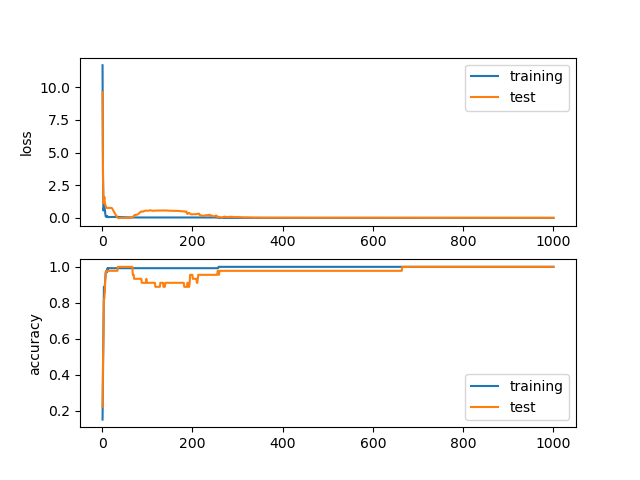
\includegraphics[width=17cm, height=10cm, keepaspectratio]{rn_plot2.png}
    \caption{Figure diagrames "accuracy" et "loss" pour réseau de neuronne a une couche cachée }
    \label{Figure diagrames "accuracy" et "loss" pour réseau de neuronne a une couche cachée }
\end{figure}  
\begin{figure}[H]
    \centering
    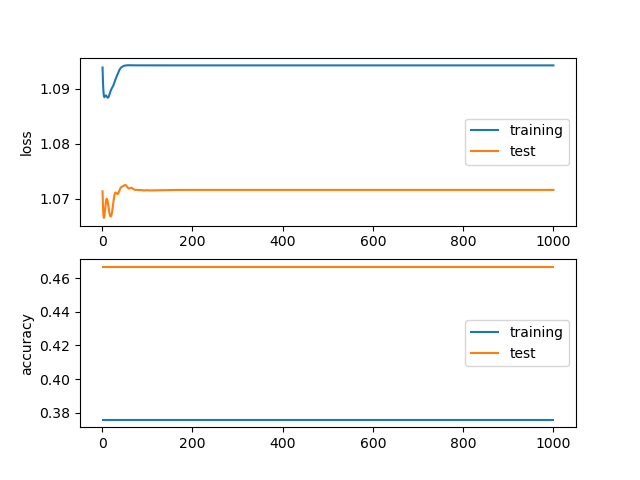
\includegraphics[width=17cm, height=10cm, keepaspectratio]{rn_plot.png}
    \caption{Figure diagrames "accuracy" et "loss" pour réseau de neuronne a deux couches cachées }
    \label{Figure diagrames "accuracy" et "loss" pour réseau de neuronne a deux couches cachées }
\end{figure}   
\par Pour "lr" entre 0.01 et 1, et pour "l2reg" entre 0.1 et 10, et pour "mu" entre 0 et 1, les meilleurs valeurs pour les hyper-paramètres "lr", "l2reg" et "mu" sont ceux affichés dans les deux figures ci-dessous
\begin{figure}[H]
    \centering
    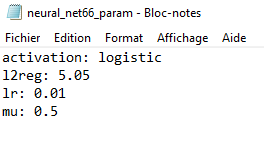
\includegraphics{rn_param_logistic.PNG}
    \caption{Figure paramètres pour réseau de neurones à deux couches cachées}
    \label{paramètres pour une fonction d'activation logistique }
\end{figure}
\begin{figure}[H]
    \centering
    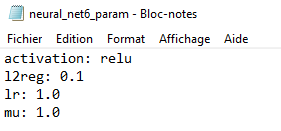
\includegraphics{rm_param_relu.PNG}
    \caption{Figure paramètres pour réseau de neurones à une couche cachée}
    \label{paramètres pour une fonction d'activation RELU }
\end{figure}
\subsection{Bagging}
\begin{figure}[H]
    \centering
    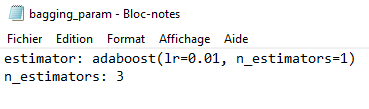
\includegraphics{bagging_param.PNG}
    \caption{Figure bagging-param }
    \label{Figure fichier bagging-param }
\end{figure}
\par Les précisions d'entrainement et de test:
\begin{figure}[H]
    \centering
    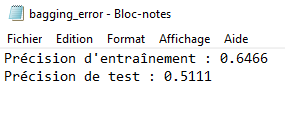
\includegraphics{bagging.PNG}
    \caption{Figure bagging-error }
    \label{Figure fichier bagging-error }
\end{figure}
\subsection{AdaBoost} 
\par Pour "lr" entre 0.01 et 1, et pour "n-estimators" entre 1 et 101, les meilleurs valeurs pour les hyper-paramètres "lr" et "n-estimator" sont ceux affichés dans la figure ci-dessous
\begin{figure}[H]
    \centering
    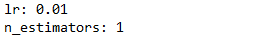
\includegraphics{adaboost_param.PNG}
    \caption{Figure adaboost-param }
    \label{Figure fichier adaboost-param }
\end{figure}
\par Les précisions d'entrainement et de test:
\begin{figure}[H]
    \centering
    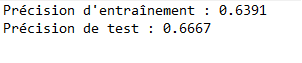
\includegraphics{adaboost.PNG}
    \caption{Figure adaboost-error }
    \label{Figure fichier adaboost-error }
\end{figure}

\section{Analyse}
\par En comparant les précisions d'entrainement et test, on constate que l'algorithme SVM a permis de faire une bonne classification par rapport aux algorithmes Bagging et Adaboost.
\par D'apres les deux graphiques correpondants à la classification par réseau de neurones, on constate que le réseau ayant deux couches cachées ne fonctionne pas alors que  celui ayant un seule couche cachée converge rapidement vers la solution optimale.
\par La classification par régression logistique converge aussi rapidement vers la solution optimale.



\end{document}

